\documentclass[a4paper,11pt,spanish]{article}

\textwidth 18.5cm
\textheight 26cm
\topmargin -2cm
\oddsidemargin -1.5cm
\parskip .3em
\parindent 0cm

%your favourite packages here
\usepackage[spanish]{babel}
% \usepackage{lineno}
% \usepackage{mathptmx}
%\usepackage{sublabel}
%\usepackage{psfrag,graphicx}
%\usepackage{subfigure}
\usepackage{amsmath}
\usepackage{amssymb}
\usepackage{amsfonts}
\usepackage{bm}
%\usepackage{bbm}
\usepackage{color}
%\usepackage{overpic}
\usepackage{latexsym}
\usepackage{epstopdf}
\usepackage{color}
%\usepackage{times}
%\usepackage{stmaryrd}

\usepackage{psfrag,graphicx}
%\usepackage{picins}
%\usepackage{epsf}
\usepackage{natbib}
\usepackage{epstopdf}\DeclareGraphicsRule{.tif}{png}{.png}{`convert #1 `basename
#1 .tif`.png}
%\usepackage{appendix}
%\usepackage{dsfont}
%\usepackage{mathtools}

\definecolor{mygrey}{gray}{0.35}
\definecolor{myblue}{rgb}{0.2,0.2,0.8}
\definecolor{myzard}{cmyk}{0,0,0.05,0}
\definecolor{mywhite}{rgb}{1,1,1}
\definecolor{myred}{rgb}{1,0.,0.3}

\def \barl {\begin{array}{rl}}
\def \ea {\end{array}}
%\definecolor{myblue}{named}{MidnightBlue}
\usepackage{hyperref}
\def\beq{\begin{equation}}
\def\eeq{\end{equation}}
\def\ba{\begin{align}}
\def\enda{\end{align}}
\def\bi{\begin{itemize}}
\def\ei{\end{itemize}}
\def\bs#1{\boldsymbol{#1}}
\def\txt#1{\textrm{#1}}

\newcommand{\eq}[1]{Eq.\;(\ref{#1})}

\newcommand{\sgn}{\operatorname{sgn}}
\def\C{{\mathbb{C}}} \def\F{{\mathbb{F}}}
\def\N{{\mathbb{N}}} \def\Q{{\mathbb{Q}}}
\def\R{{\mathbb{R}}} \def\Z{{\mathbb{Z}}}
\def\cH{{\mathcal H}}
\def\bfsigma{\boldsymbol{\sigma}}
\def\bfmu{\boldsymbol{\mu}}
\def\dd{\mathord{\rm d}} \def\Det{\mathop{\rm Det}}
\def\dist{\mathop{\rm dist}} \def\ee{\mathord{\rm e}}
\def\End{\mathord{\rm End}} \def\ev{\mathord{\rm ev}}
\def\id{\mathord{\rm id}} \def\ii{\mathord{\rm i}}
\def\min{\mathord{\rm min}} \def\mod{\mathord{\rm mod}}
\def\prob{\mathord{\rm prob}}
\def\tr{\mathop{\rm Tr}}
\def\half{\textstyle\frac{1}{2}}
\def\third{\textstyle\frac{1}{3}}
\def\fourth{\textstyle\frac{1}{4}}

\graphicspath{{figs/}}

\newcommand{\da}{\downarrow}
\newcommand{\ua}{\uparrow}

\renewcommand{\ii}{{\rm i}}
\renewcommand{\ee}{{\rm e}}

%brackets
 \newcommand{\ket}[1]{|#1\rangle}
 \newcommand{\bra}[1]{\langle #1|}
 \newcommand{\braket}[2]{\langle #1|#2\rangle}

 \newcommand{\ketbra}[2]{\ket{#1}\bra{#2}}
 \newcommand{\proj}[1]{\ketbra {#1}{#1}}
 \newcommand{\biket}[2]{\ket{#1\;#2}}
 \newcommand{\bibra}[2]{\bra{#1\;#2}}
 %\newcommand{\ketbradif}[2]{\biket {#1}{#2}\bibra {#1}{#2}}
% \newcommand{\preespacio}{\!\text{\hspace{0.2 ex}}}
% \newcommand{\postespacio}{\!\text{\hspace{0.75 ex}}}


% \graphicspath{{Plots/}}

\begin{document}

%\title[Short Title]{Ejercicios para el curso de Introducci\'on a la \'Optica Cu\'antica}

\author{C. Cormick}

% \maketitle

\noindent{\large \bf Procesamiento Cu\'antico de la Informaci\'on - C. Cormick, FING - 1er sem. 2025}\\

\noindent{\large \bf Práctico 3 - Formalismo matemático de información cuántica}\\

\vspace{20pt}


\begin{enumerate}
   \item {\bf Producto interno.} (Repaso para quien lo necesite.)\\
   El producto interno de dos vectores columna complejos $\vec v, \vec w$ de dimensión arbitraria $d$ se define como:
  $$(\vec v, \vec w ) = (\vec v)^\dagger \cdot \vec w = \sum_{j=1}^d v_j^* w_j$$
  donde $v_j$, $w_j$ indican las componentes de los vectores, el operador ``$\dagger$'' denota el transpuesto conjugado, y el asterisco indica conjugado. Ojo, el orden de los vectores no da lo mismo! La norma de un vector es la ra\'iz cuadrada de su producto interno consigo mismo. Dos vectores se dicen ortogonales si su producto interno es cero. Dados los vectores 
$$ \left(\barl 1+i\\ -1~\\ 0 ~\ea \right), \left(\barl 1\\ i\\ 0 \ea \right), \left(\barl 3\\ 2\\ 1 \ea \right)
$$
calcular los productos internos entre cada par de vectores y tambi\'en las normas de los tres vectores.
\smallskip

 \item {\bf Compuertas como matrices unitarias.} \\
 Las compuertas cu\'anticas est\'an representadas por matrices unitarias, que satisfacen la propiedad $U^\dagger = U^{-1}$, o sea que $U U^\dagger = U^\dagger U = \mathbb{I}$, donde la daga indica el transpuesto conjugado.
 
 \begin{enumerate}
  \item Mostrar que los autovalores de las matrices unitarias deben tener m\'odulo 1.
  \item Mostrar que las matrices unitarias preservan el producto interno, esto es, si $U$ es unitaria el producto interno entre dos vectores $\vec v$ y $\vec w$ es igual al producto entre los vectores $U\vec v$ y $U\vec w$.
 \end{enumerate}

  \item {\bf \'Algebra lineal - 1 qubit.} El espacio de estados de un qubit es un espacio vectorial de dimensi\'on 2, con una base dada por: $\{\vec e_0, \vec e_1\}$, donde: 
  $$\vec e_0 = \begin{pmatrix}
                1\\0
               \end{pmatrix}
               \quad\quad               
    \vec e_1 = \begin{pmatrix}
                0\\1
               \end{pmatrix}$$ 
 A cada vector $\vec e_j$ lo asociamos con el estado cl\'asico correspondiente al qubit blanco ($j=0$) y negro ($j=1$). 
  
  El estado neblinoso de un qubit dado por:
  \begin{center}
   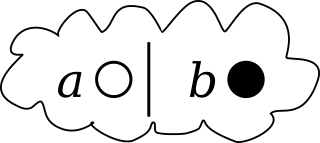
\includegraphics[width=60pt]{1qubit_state.png}
  \end{center}

  puede expresarse entonces como el vector $a \vec e_0 + b \vec e_1$, donde $a,b\in\mathbb{C}$. El estado se dice normalizado cuando $|a|^2+ |b|^2=1$. Las compuertas que act\'uan sobre un qubit se escriben como matrices que operan sobre los vectores columna; para corresponder a transformaciones f\'isicas, estas matrices deben ser {\it unitarias}, lo que implica que son inversibles y preservan el producto interno.
  
  \begin{enumerate}
   \item Si el estado es de la forma $a \vec e_0 + b \vec e_1$, indicar su forma en notación matricial y cuál es la probabilidad de medir 0 y 1. 
   
   \item Escribir la forma matricial de las compuertas: $X$, $H$, $Z$. Mostrar que todas ellas son su propia inversa.
   
   \item Demostrar usando productos matriciales las siguientes propiedades: $ZX=-XZ$, $HXH=Z$.
   
   \item Escribir cu\'ales son los autoestados / vectores propios de $X$ y de $Z$ indicando sus correspondientes valores propios.
  \end{enumerate}
  
    \item {\bf Matrices de Pauli.} Adem\'as de los operadores correspondientes a las compuertas $X$ y $Z$, se define un operador $Y$ sobre un qubit en la forma: 
    $$Y = \begin{pmatrix} 0 & -i \\ i & ~0\end{pmatrix}$$ 
    Los tres operadores $X, Y, Z$ se conocen como ``matrices de Pauli''. 
 \begin{enumerate}
  \item Verificar que se trata de una operaci\'on unitaria y que adem\'as es su propia inversa (igual que $X$ y $Z$).
  
  \item Hallar los vectores y valores propios de $Y$.
  
  \item Probar que se satisface $XY = -YX$, $YZ = -ZY$ (ya sab\'iamos que $ZX=-XZ$); se dice que las matrices de Pauli ``anticonmutan''.
  
  \item Verificar que $XY = {\rm i} Z$, $Y Z = {\rm i} X$, $ZX = {\rm i} Y$ (notar que el orden de los operadores cambia c\'iclicamente).
  
  \item Mostrar que $HYH=-Y$.
 \end{enumerate}
\smallskip

\item {\bf Esfera de Bloch.}

Una forma de representar un estado (puro) de un qubit es como un vector $\vec a$ de norma 1 que indica que el estado en cuestión es el autovector de autovalor +1 del operador $1/2\, (\mathbb{I} + a_x X + a_y Y + a_z Z)$, donde $\vec a$ es el
``vector de Bloch'', y $X, Y, Z$ son las matrices de Pauli.
\begin{enumerate}
 \item Mostrar que con esa definición, los estados computacionales $\vec e_0$ y $\vec e_1$ corresponden a flechas que apuntan hacia arriba y abajo respectivamente.
 \item De la misma forma, mostrar cuál es la representación de Bloch de los estados $\vec v_{\pm} = (\vec e_0 \pm \vec e_1)/\sqrt{2}$.
 \item La aplicación de cualquier compuerta unitaria de un qubit es equivalente a una rotación en la esfera de Bloch. \textquestiondown A qué rotación corresponde la compuerta de Hadamard?
\end{enumerate}

\smallskip


\item {\bf \'Algebra lineal - 2 qubits.} El espacio de estados de un sistema de $n$ qubits es un espacio vectorial complejo de dimensi\'on $2^n$. Una base del espacio de estados puede tomarse como $\{\vec e_j,\, j=0,1,\ldots, 2^n-1\}$ donde la representaci\'on binaria del n\'umero entero $j$ indica el estado de cada qubit (blanco en 0, negro en 1). Los vectores de esta base se toman como ortonormales. Consideramos a continuaci\'on el caso de 2 qubits.
  
  \begin{enumerate}
   \item Escribir expl\'icitamente la descomposici\'on binaria de los n\'umeros del 0 al 3. Para poder comparar, fijamos la convención de que el primer (segundo) elemento de esta descomposición indicará el estado del primer (segundo) qubit (en algunos contextos esto se elige al revés, y da igual, pero hay que ser conciente de la convención usada). Dibujar la representación gráfica que corresponde a cada estado. Escribir tambi\'en expl\'icitamente la forma de los cuatro vectores columna correspondientes a los $\vec e_j$, y notar que esta forma no tiene nada que ver con la descomposici\'on binaria de $j$.
   \item Si el estado es de la forma $\vec v = \sum a_j \vec e_j$, escribir qu\'e condici\'on deben satisfacer los coeficientes para que el estado est\'e normalizado. Indicar la probabilidad de hallar el primer qubit en cero/blanco. Repetir para el segundo qubit.
   \item Indicar la representaci\'on matricial de las compuertas de 2 qubits $SWAP$, $CZ$, $CNOT_{12}$ y $CNOT_{21}$. Mostrar que cada una de ellas es su propia inversa.
   \item Escribir la representaci\'on matricial en el espacio de 2 qubits de la operaci\'on $X$ sobre el primer qubit y sobre el segundo (dejando en cada caso el otro qubit sin alterar). 
   
   \item A partir del ítem anterior, mostrar que aplicar una compuerta $X$ sobre un qubit acompa\~nada de la identidad sobre el otro qubit se puede escribir como un producto de Kronecker de las correspondientes matrices de 2$\times$2. 
   
   Nota 1: Esto vale para cualquier compuerta de la forma $A\otimes B$, y no es una casualidad, sino una consecuencia de elegir la base de vectores del espacio compuesto como el producto tensorial de las bases individuales.
   
   Nota 2: Si se numeran los qubits en orden de izquierda a derecha en la descomposición binaria, la representaci\'on matricial de la operación $A_1\otimes B_2$ queda:
   $${\displaystyle \mathbf {A} \otimes \mathbf {B} ={\begin{bmatrix}a_{11}\mathbf {B} & a_{12} \mathbf {B} \\ a_{21}\mathbf {B} & a_{22} \mathbf {B} \end{bmatrix}},}$$
   Si la numeración de los qubits es al revés se intercambian los roles de A y B al armar la matriz de 4x4.
   
   \end{enumerate}
   
   \item {\bf Composici\'on de compuertas de 2 qubits.}
   
   \begin{enumerate}
   \item Demostrar por medio de operaciones matriciales que la composici\'on de compuertas $(I_1 \otimes H_2)\, CZ \, (I_1 \otimes H_2)$ es efectivamente igual a un $CNOT_{12}$ donde el primer qubit es el control y el segundo es el target (este es el problema 10 del práctico 1).
   
   \item Realizar ahora las operaciones matriciales correspondientes a la concatenaci\'on de tres compuertas $CNOT_{12} \, CNOT_{21}\, CNOT_{12}$, como en el problema 15 del práctico 1, y verificar el resultado obtenido anteriormente.
  \end{enumerate}

  \item {\bf Phase kick-back.} Dado un sistema de un qubit, llamamos $\vec v_{\pm}$ a los autoestados (de norma 1) de la compuerta $X$ con autovalor $\pm 1$ respectivamente (recordar el problema 5). Cuando el estado de un sistema de dos qubits es separable, podemos usar la notaci\'on $\vec v \otimes \vec w$ donde el primer/segundo vector corresponde al primer/segundo qubit. 
  \begin{enumerate}
   \item Considerar los estados de la forma $\{\vec v_{\pm}\otimes \vec v_{\pm}\}$ (donde cada signo es independiente, son cuatro estados en total). Mostrar que son autoestados de los operadores $A=X\otimes\mathbb{I}$ y $B=\mathbb{I}\otimes X$, y calcular los autovalores.
   \item Calcular el efecto de la compuerta $CNOT_{12}$ sobre esos cuatro estados. Notar que este es el truco que se usa en el algoritmo de Deutsch.
  \end{enumerate}
  
  \item {\bf Estados de Bell.} (Contin\'ua el problema del práctico 2).
  
  \begin{enumerate}
   \item Escribir la forma vectorial de los cuatro estados de Bell.
   \item Escribir la forma matricial del circuito creador de estados de Bell.
   \item Verificar por medio de operaciones matriciales las transformaciones del problema 4 del práctico 2.
  \end{enumerate}

 \item {\bf Estados de $n$ qubits.} Considere el estado de $n$ qubits dado por $\vec v = \sum_j c_j \vec e_j$ donde $j\in\{0,1,\ldots,2^n-1\}$. Indicar:
 \begin{enumerate}  
  \item Qué condición deben cumplir los coeficientes para que el estado esté normalizado.
  \item Cu\'ales son los valores de los coeficientes $c_j$ si el estado considerado es el $\vec e_l$ (con $l$ un entero arbitrario entre 0 y $2^{n-1}$).
  \item Qu\'e condici\'on debe cumplirse para que el estado considerado sea ortogonal al $\vec e_l$.
  \item Cuál es la probabilidad de que al medir el primer qubit se obtenga un cero.
  \item Cuál es la probabilidad de que al medir el último qubit se obtenga un cero.
  \item Cu\'ales son los valores de los coeficientes $c_j$ si el estado considerado es el $H^{\otimes n} \vec e_0$, donde $H^{\otimes n}$ es el operador que aplica compuertas de Hadamard sobre los $n$ qubits a la vez.
  \item Qu\'e condici\'on debe cumplirse para que el estado sea ortogonal a $H^{\otimes n} \vec e_0$.
  \end{enumerate}
  
  \item {\bf Transformada de Hadamard.} Considerar el operador $H^{\otimes n}$ actuando sobre un sistema de $n$ qubits. Mostrar que:
  $$H^{\otimes n}\, \vec e_j = \frac{1}{\sqrt{2^n}} \sum_{l=0}^{2^n-1} (-1)^{\vec j \cdot \vec l}\, \vec e_l$$
  donde llamamos $\vec j$ y $\vec l$ a los arreglos de $n$ bits correspondientes a la descomposición binaria de los números $j$ y $l$ respectivamente, de modo que $\vec j \cdot \vec l = j_1 l_1 + \cdots + j_n l_n$.

  {\it Ayuda: Puede ser útil comenzar con el caso de solo dos qubits y luego generalizar a $n$ arbitrario.}

\end{enumerate}

\end{document}
